% Pacotes e configurações padrão do estilo ``article''\
% -------------------------------------
\documentclass[a4paper,11pt]{article}
% Layout
% ------------------------------------------------------------------------------
%     Gráficos e layout ----------------------------------------------------------------------

\ifx\pdfmatch\undefined
\else
    \usepackage[T1]{fontenc}
    \usepackage[utf8]{inputenc}
\fi
% xetex:
\ifx\XeTeXinterchartoks\undefined
\else
    \usepackage{fontspec}
    \defaultfontfeatures{Ligatures=TeX}
\fi
% luatex:
\ifx\directlua\undefined
\else
    \usepackage{fontspec}
\fi
% End engine-specific settings

%      Fonte --------------------------------------------------------------------------------
%\usepackage{lmodern}
\usepackage{times}
%     Pacotes adicionados -------------------------------------------------------------------
\usepackage{ae}
%     Língua e hifenização ------------------------------------------------------------------
\usepackage[portuguese]{babel}
\usepackage{hyphenat}
%      Outros --------------------------------------------------------------------------------
\usepackage{hyperref} % Permite Links personalisados usando hyperref
\usepackage{fancyhdr}
\usepackage{sectsty}
\usepackage{float}   % Gerencia melhor o posicionamento das figuras e tabelas
%\usepackage{graphicx}
\usepackage[pdftex]{color,graphicx}
\usepackage{hyperref}
\usepackage{enumerate} % Permite alterar Layout do enumerate
%\usepackage{pdflscape}  % Permite alterar a orientação da pagina para Paisagem
%\usepackage{ifthen}  % Permite usar condicionais ifelse
%\usepackage[table]{xcolor} % Permite alterar as cores das células de uma tabela
\usepackage{amsmath,amssymb} % Ambiente para uso de elementos matemáticos
\usepackage{caption}
\usepackage{subcaption} % permite o uso de multiplas figuras com legenda (ambiente subfigure)
%\usepackage{minted} % Ambiente minted para colorir código de programas
\usepackage{natbib} % Para referencia bibliográfica
\usepackage{url}    % Referência de links na internet
%\usepackage{listings} % pacote para apresentar código de programação
\usepackage{indentfirst}  % Para indentar o primeiro parágrafo de cada seção
\usepackage{titling}  % Permite Montar uma página de titulo própria

% Layout do documento ------------------------------------------------------------------------
%     Bordas e tamanho da página ------------------------------------------------------------
\usepackage{geometry} 
 \geometry{ % Padrõa ABNT para relatórios
 a4paper,
 left=30mm,
 right=20mm,
 top=30mm,
 bottom=20mm
 }
%     Cabeçalho e Rodapé ---------------------------------------------------------------
\pagestyle{fancy}
  \lhead{}
  \chead{}
  \rhead{}
  \lfoot{}
  \cfoot{}
  \rfoot{\thepage}
%     Númeração ------------------------------------------------------------------------
  \pagenumbering{arabic}
%     Retas do cabeçalho e rodapé ------------------------------------------------------
  \renewcommand{\headrulewidth}{0.5pt}
  \renewcommand{\footrulewidth}{0.5pt}
%     Tamanho da letra de seções e derivadas --------------------------------------------
  \sectionfont{\normalsize}
  \subsectionfont{\small}
%     Hiperlinks ------------------------------------------------------------------------
  \hypersetup{
                  colorlinks,
                  citecolor=black,
                  filecolor=black,
                  linkcolor=black,
                  urlcolor=black
                  }
%     Definições do pdf ----------------------------------------------------------------------
\hypersetup{
    unicode=false,          % non-Latin characters in Acrobat’s bookmarks
    pdftoolbar=true,        % show Acrobat’s toolbar?
    pdfmenubar=true,        % show Acrobat’s menu?
    pdffitwindow=false,     % window fit to page when opened
    pdfstartview={FitH},    % fits the width of the page to the window    
    pdfauthor={Rafael Lima},     % author
    pdfnewwindow=true      % links in new window
}
%     Outros ----------------------------------------------------------------------------
      %\renewcommand{\thesection}{(\alph{section})} % muda o estilo de númeração das sections
      % alterando a formatação dos numeradores de lista de itens
      \renewcommand\theenumi{\arabic{enumi}}
      \renewcommand\labelenumi{(\textit{\theenumi})}
	  \renewcommand\theenumii{\arabic{enumii}}
	  \renewcommand\labelenumii{(\textit{\theenumi.\theenumii})}
      
% ---------------------------------------------------------------------------------------


%\usepackage{circuitikz}
\usepackage[makestderr]{pythontex}

\title{Laboratório 3} % Define o título do Relatório
\author{Rafael Lima}

% Definições Auxiliares ( Macros próprias )
% ------------------------------------------------------------------------------
%\input{relat_aux.tex} % Arquivo com minhas macros
\newcommand{\npy}[1]{\sympy{round(#1,4)}}
% ----------------------------------~>ø<~---------------------------------------
\begin{document}
% Capa e Índice ----------------------------------------------------------------
%--------------------------------------------------- Capa --------------------------------------------
%\newpage
\begin{figure}[h!]
\centering

\includegraphics[scale=0.9]{img/simb_unb.png}
\label{fig:unb}
\end{figure}

\begin{center}
{\LARGE Universidade de Brasília}\\
Departamento de Engenharia Elétrica\\
Professor: Henrique Cezar Ferreira\\
Disciplina: Controle Digital\\
\end{center}


\vspace{0.18\textheight}

\begin{center}
    \Huge \textbf{\\\thetitle \\}
\end{center}

\vspace*{\fill} % Completa espaço em branco e empurra o resto para o final da página

% Tabela com os nome das pessoas do grupo

\begin{table}[H]
    \begin{tabular}{ll}
        % Nome      & Matrícula
        Rafael Lima & 10/0131093 \\
    \end{tabular}
\end{table}

\vspace{0.5cm}

\begin{center}
    \textbf{Brasília\\
    \the\year} % Coloca o Ano atual
\end{center}

\thispagestyle{empty} % Retira o cabeçalho e o rodapé da página

% ------------------------------------------------- Índice -------------------------------------------
\newpage
\tableofcontents
\newpage
% ----------------------------------------------------------------------------------------------------

 % Capa para UnB
% Conteúdo ---------------------------------------------------------------------

\section{Controle Proporcional em Tempo Discreto}

% Código fonte colocado a parte para facilitar validação dentro do ipython
\begin{sympycode}
# Get Source Code
sys.path.insert(1, '../../')
from src.python.exsim3 import *
\end{sympycode}

Dado o controlador $G_c(s)$ definido por

\begin{equation}
    G_c(z) = \sympy{sGc}
\end{equation}

Temos que $G(z)$

\begin{equation}
    G(z) = \sympy{sGz}
\end{equation}

Logo a $G_{ma}(z)$

\begin{equation}\label{eq:ex3-gma1}
    G_{ma}(z) = \sympy{sGma}
\end{equation}

A partir do qual temos a seguinte função de transferência em malha fechada

\begin{equation}
    G_{mf}(z) = \sympy{sGmf}
\end{equation}

Em que o polinômio característico é dado por

\begin{equation}
    \phi(z) = \sympy{poly}
\end{equation}

Isolando $K$ temos

\begin{equation}\label{eq:ex3-k-poly}
    K(z) = \sympy{sK}
\end{equation}

\subsection{LGR}

Avaliando a função para diferentes períodos de amostragem obtemos os seguintes gráficos do lugar das raízes para a função de transferência de malha aberta $G_{ma}(z)$ dada pela equação \ref{eq:ex3-gma1}.

\begin{figure}[H]
    \centering
    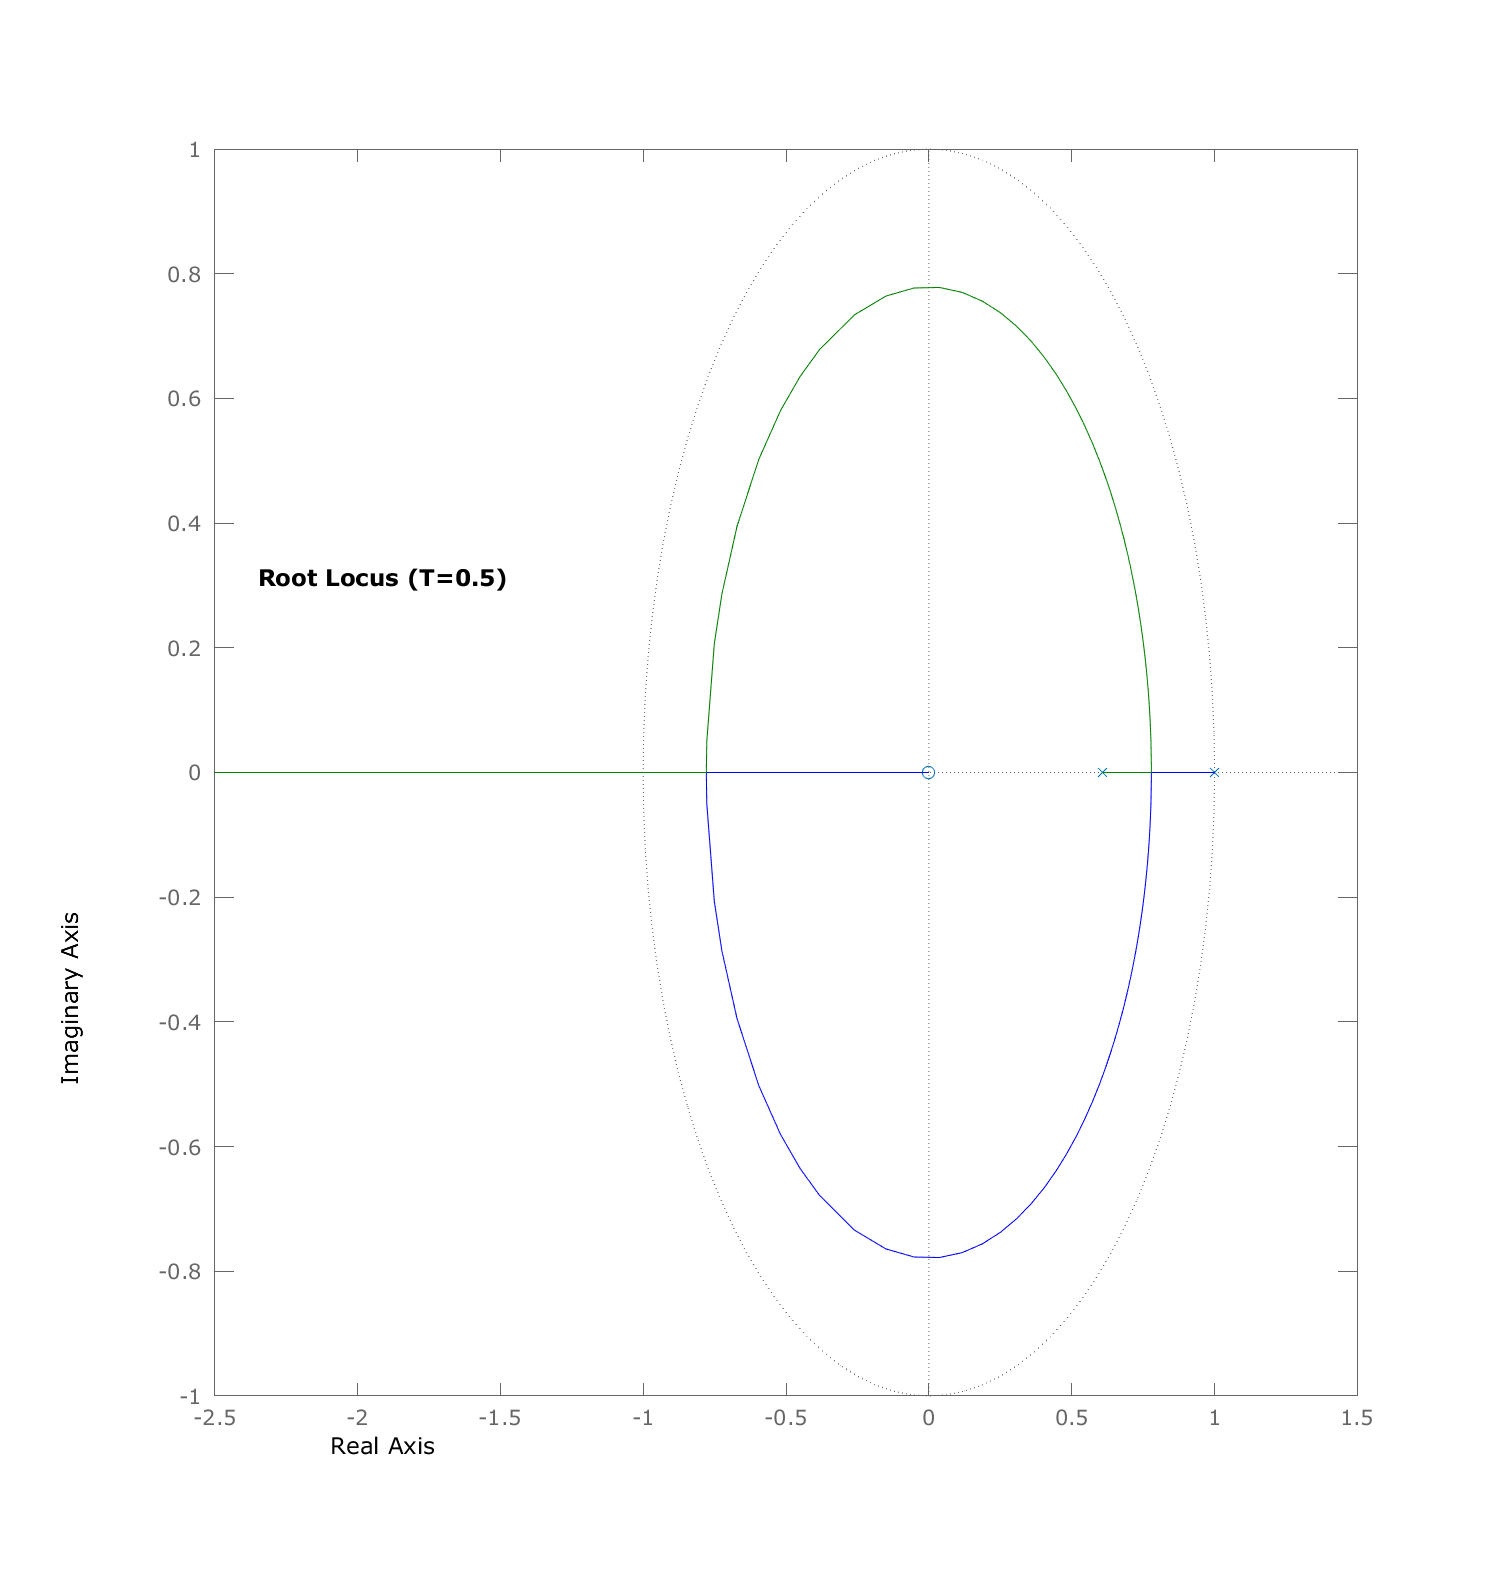
\includegraphics[width=0.9\linewidth]{img/exsim3-rlocus-t500ms.png}
    \caption{ $T=0.5s$}
\end{figure}

\begin{figure}[H]
    \centering
    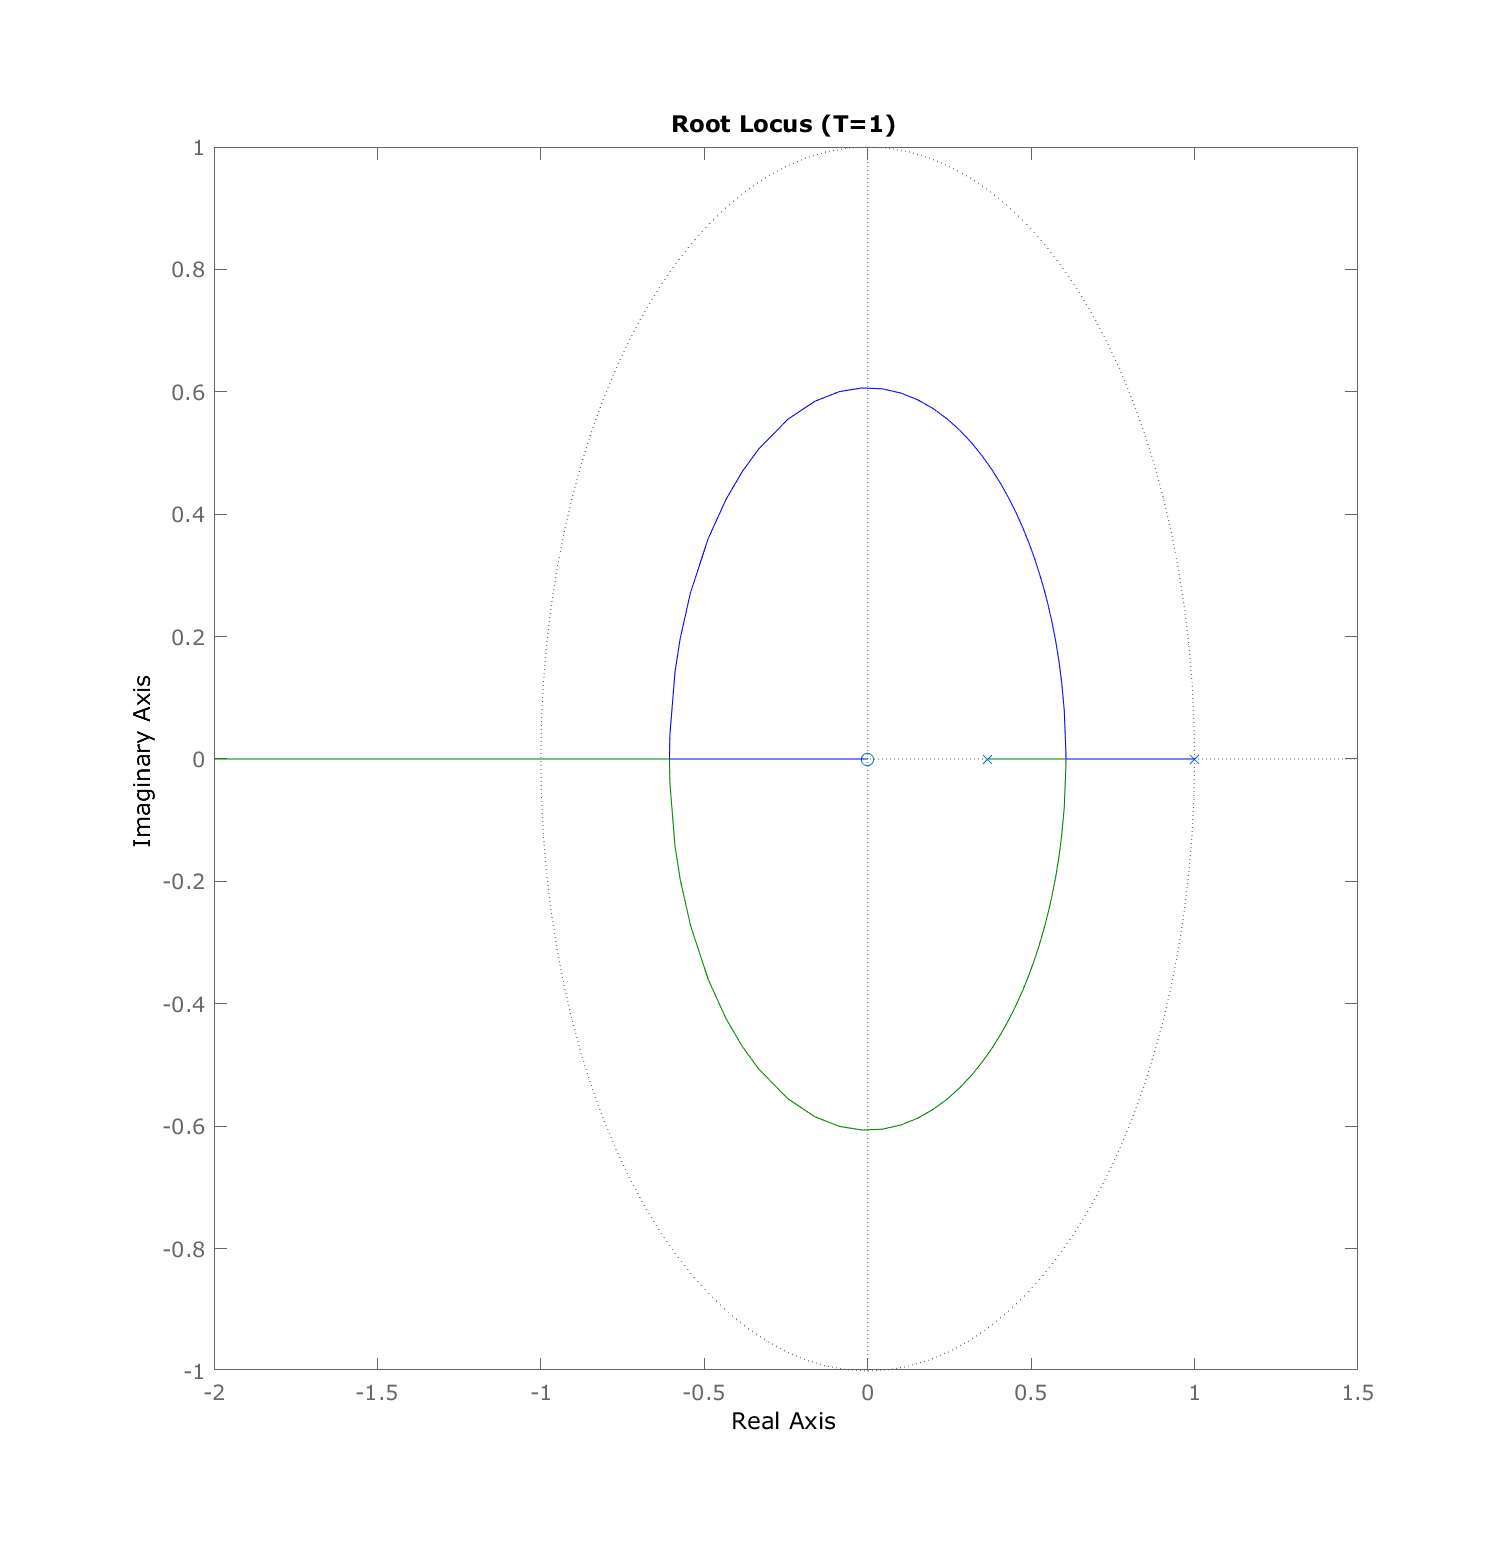
\includegraphics[width=0.9\linewidth]{img/exsim3-rlocus-t1000ms.png}
    \caption{ $T=1s$}
\end{figure}

\begin{figure}[H]
    \centering
    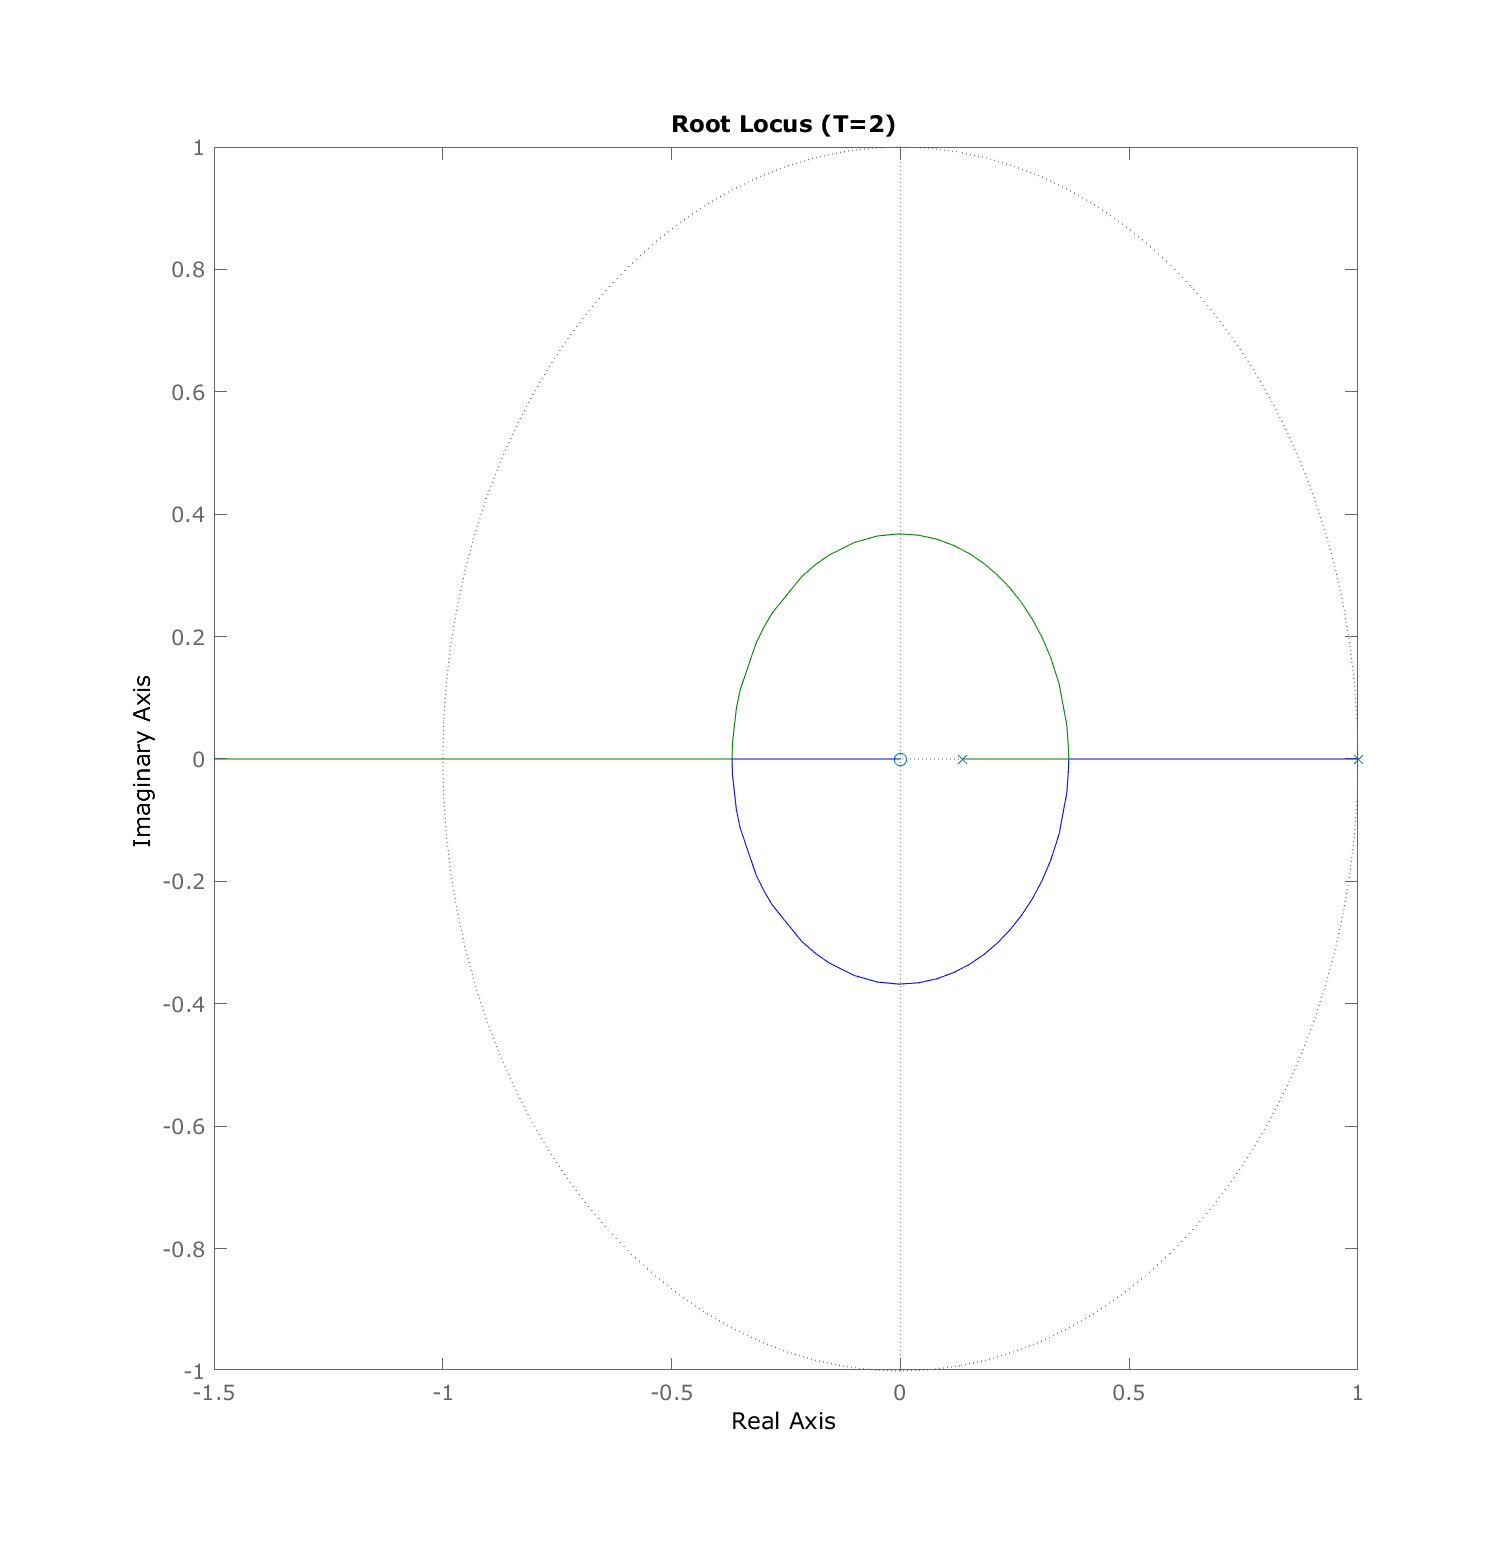
\includegraphics[width=0.9\linewidth]{img/exsim3-rlocus-t2000ms.png}
    \caption{ $T=2s$}
\end{figure}

Pelas figuras nota-se que o gráfico do LGR cruza o circulo de raio unitário definido em tracejado apenas no ponto $z=-1$ de modo que, em particular para este sistema podemos encontrar o valor do ganho crítico subsituindo $z=-1$ na equação \ref{eq:ex3-k-poly}. Em particular para $T=\{0.5,1,2\}$ temos os seguintes valores críticos para $K$:

\begin{table}[H]
    $$
    \begin{array}{cl}
        \hline
        T [ms] & K_{max} \\
        \hline
        0.5 & \npy{sK.subs([(T,0.5),(z,-1)])}\\
        1 & \npy{sK.subs([(T,1),(z,-1)])}\\
        2 & \npy{sK.subs([(T,2),(z,-1)])}\\
        \hline
    \end{array}
    $$
\end{table}

\subsection{Resposta ao Degrau} 

Simulando o sistema para diferentes os períodos de amostragem $T={0.5,1,2}$ foram obtidos respectivavamente as seguintes respostas.

\begin{figure}[H]
    \centering
    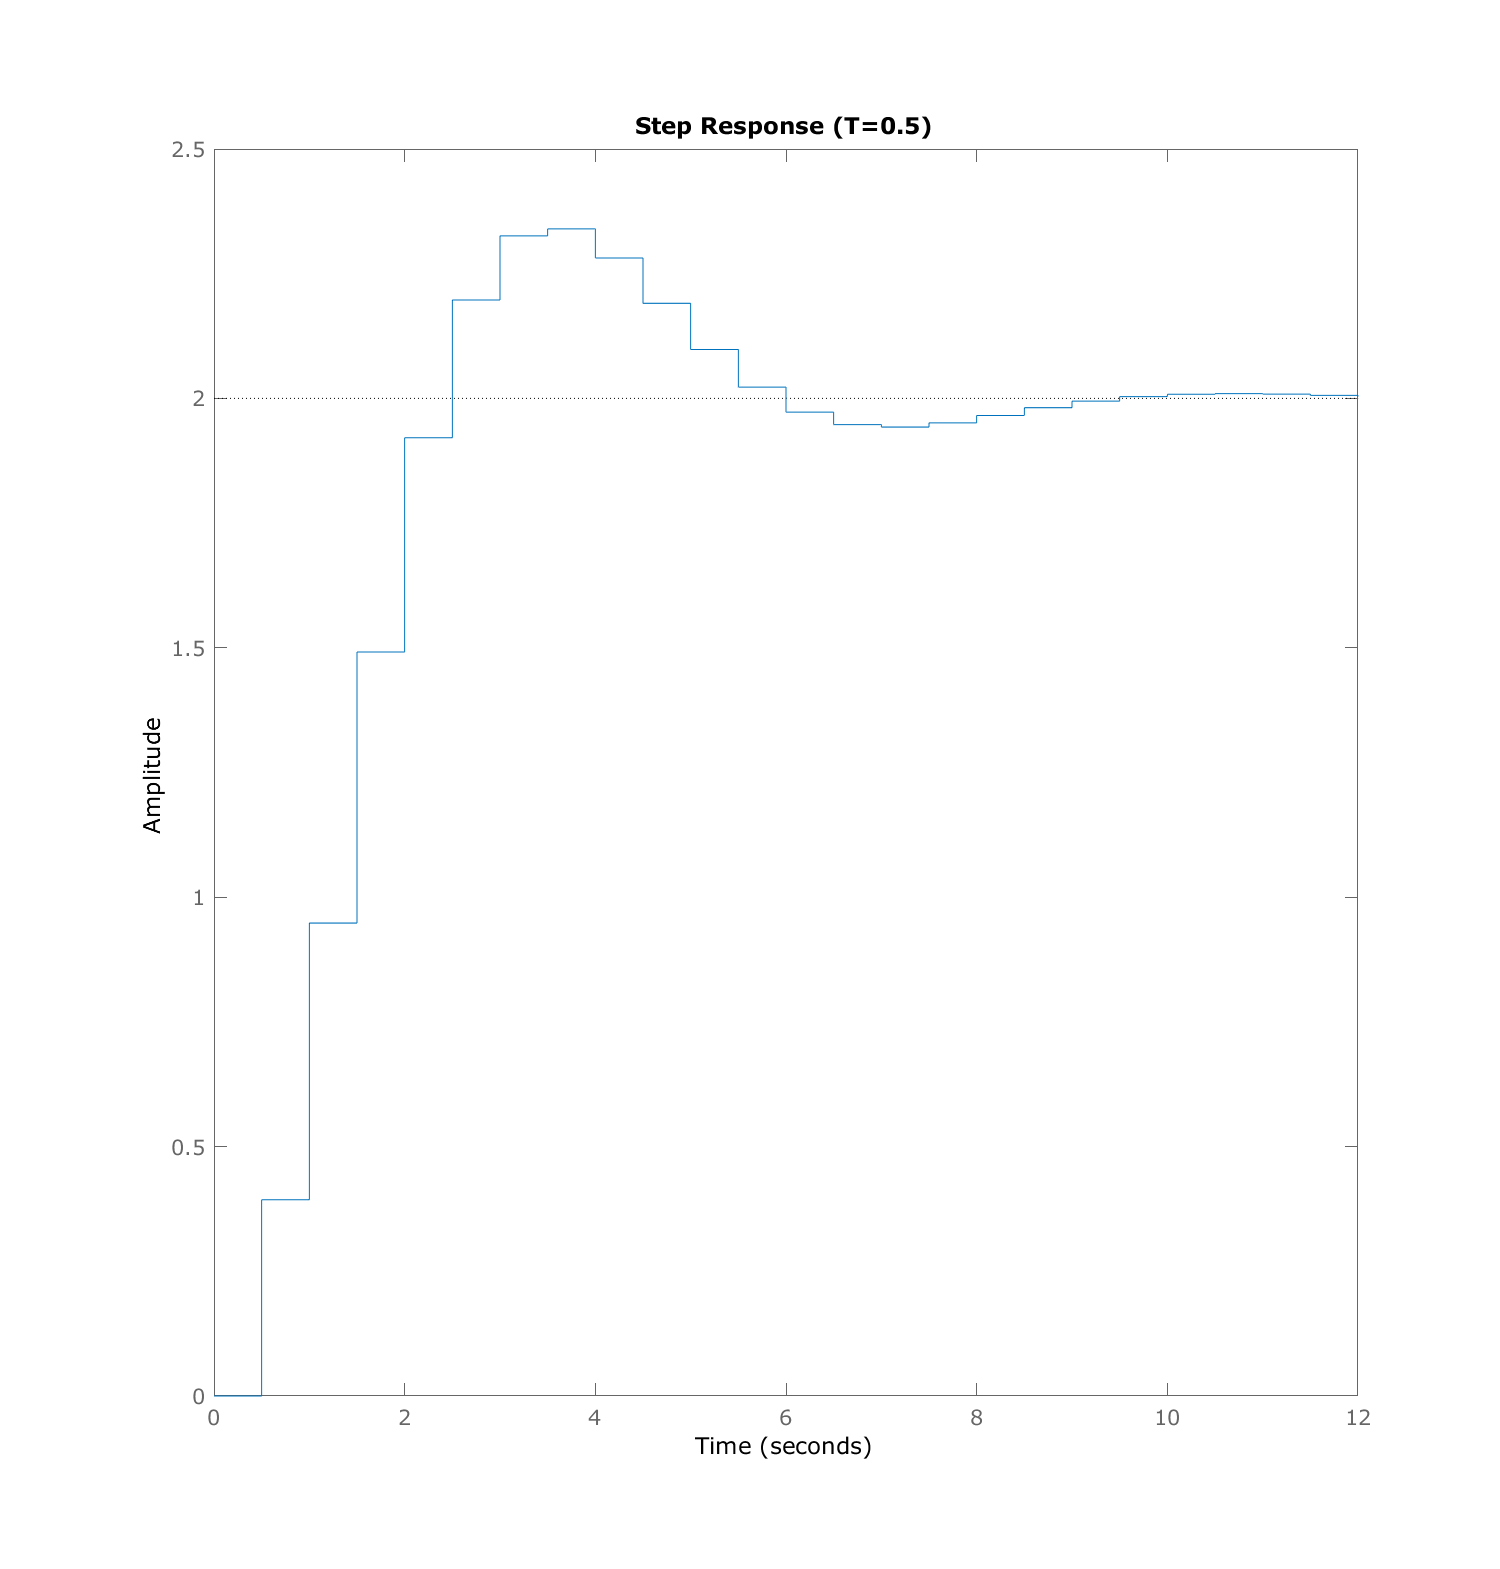
\includegraphics[width=0.8\linewidth]{img/exsim3-step-t500ms.png}
    \caption{ $T=0.5s$}
\end{figure}

\begin{figure}[H]
    \centering
    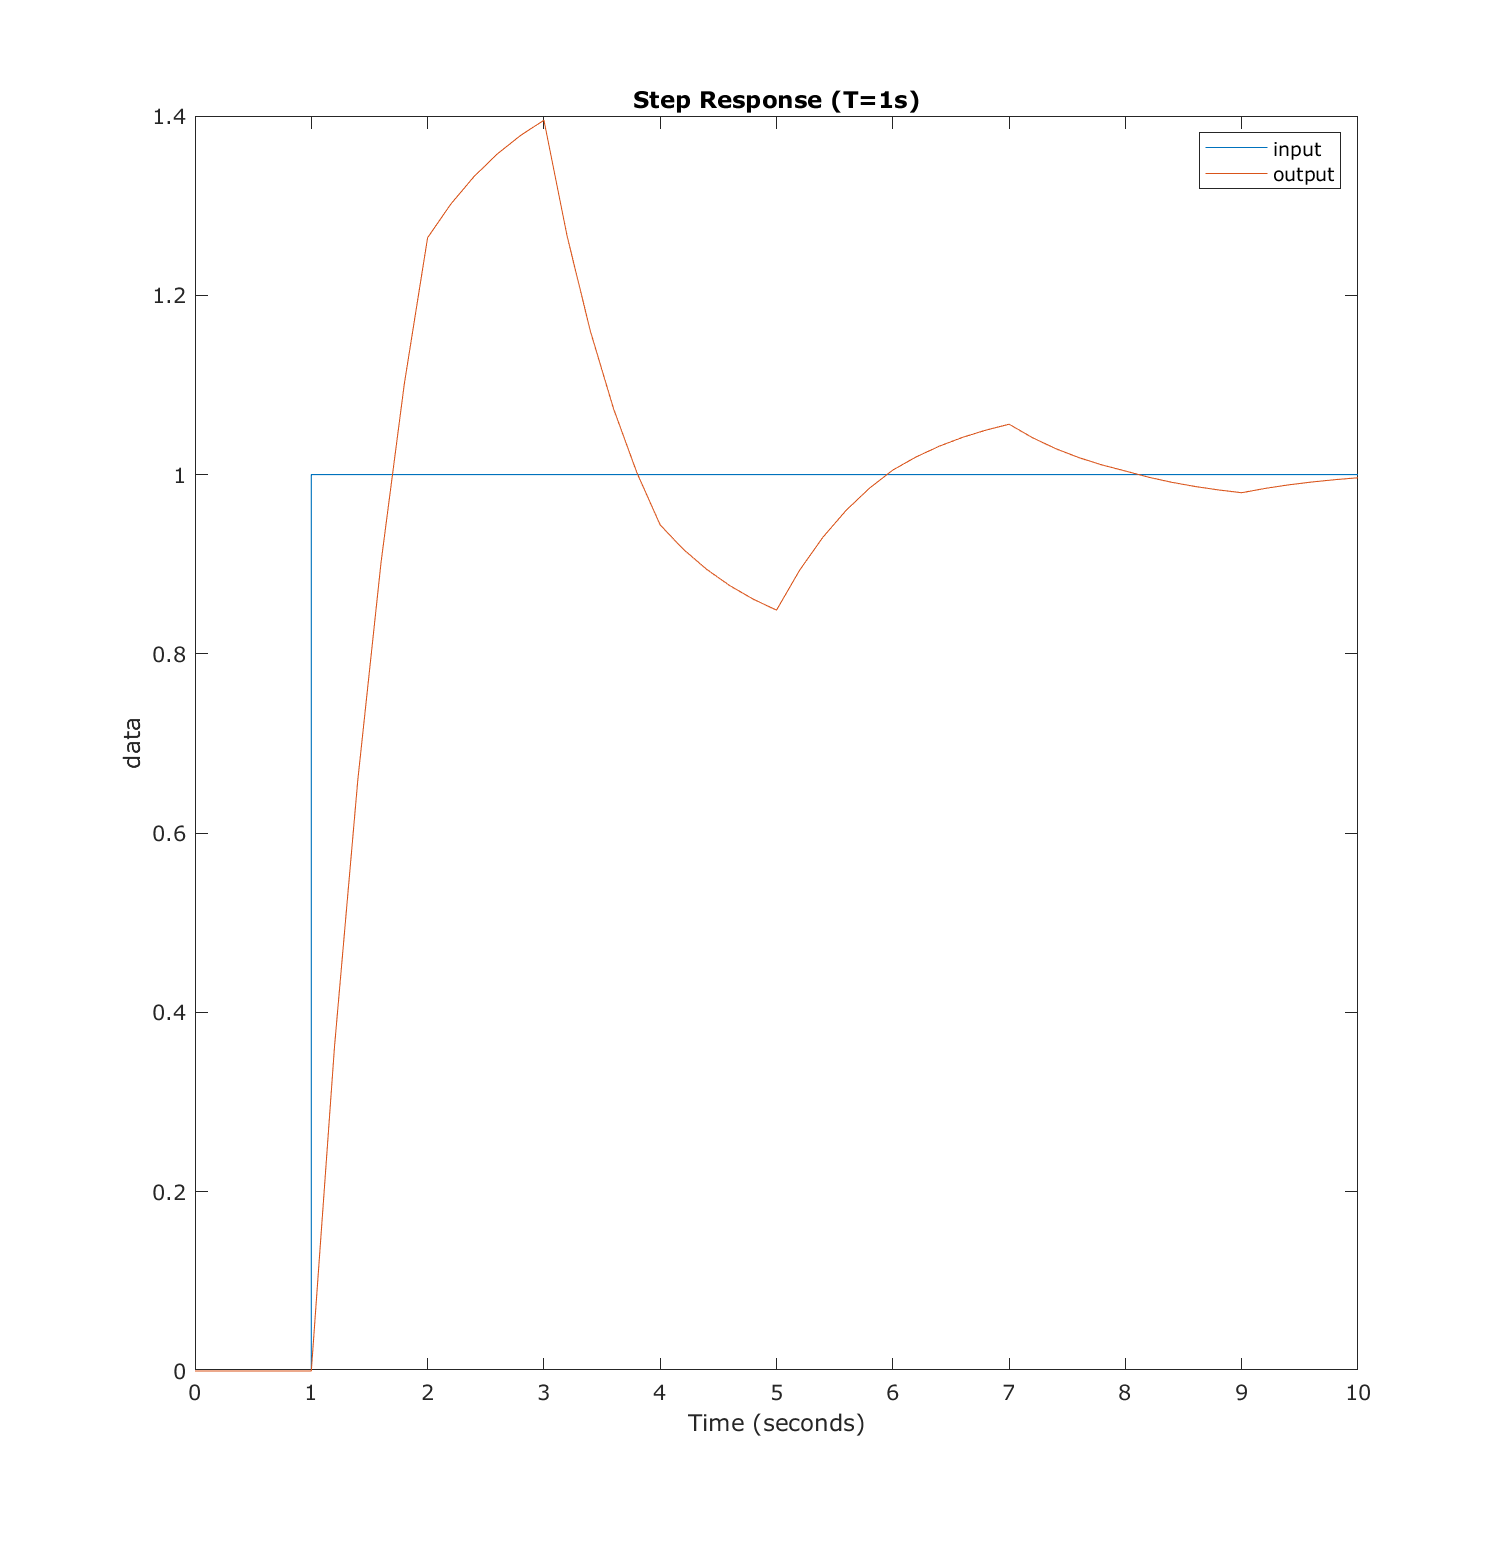
\includegraphics[width=0.8\linewidth]{img/exsim3-step-t1000ms.png}
    \caption{ $T=1s$}
\end{figure}

\begin{figure}[H]
    \centering
    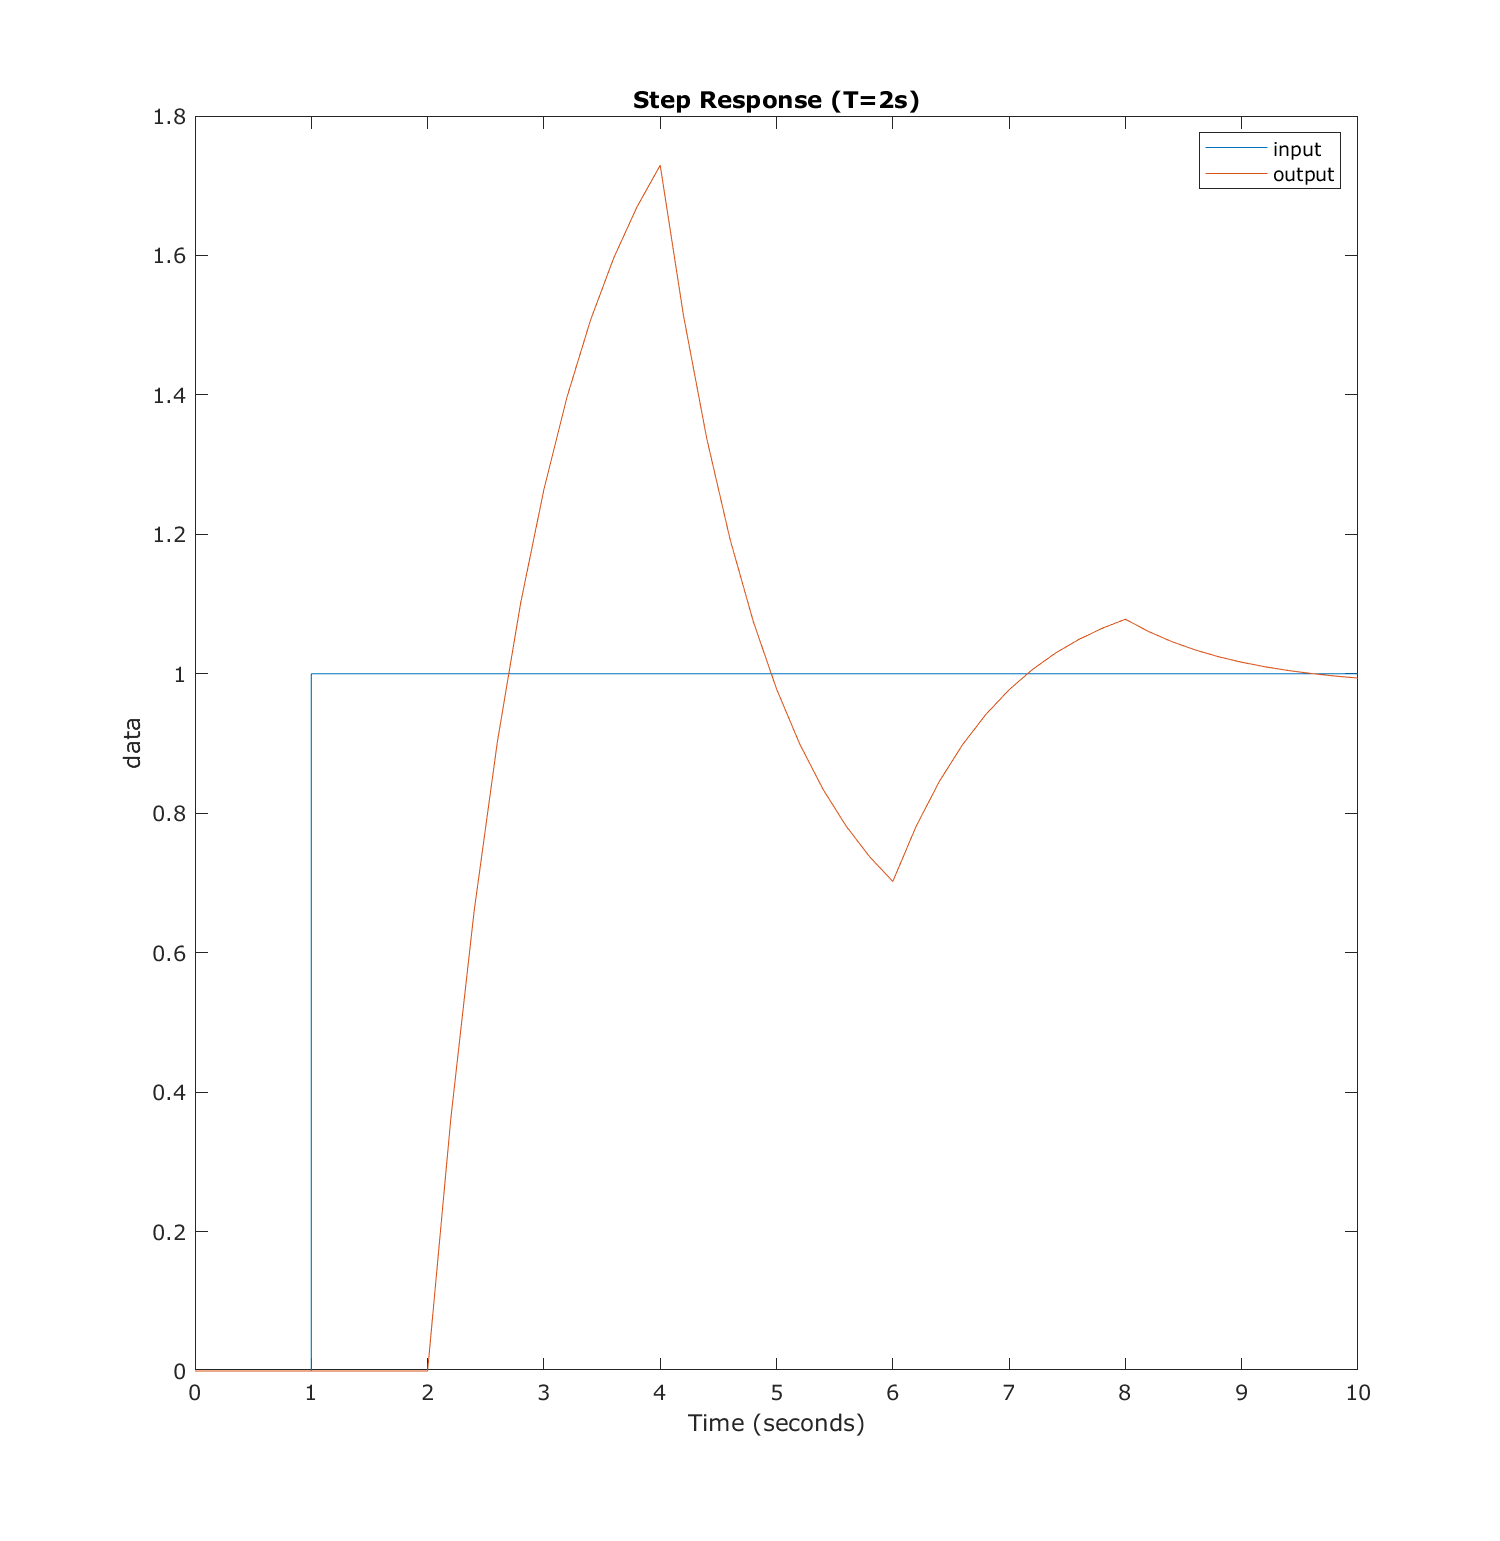
\includegraphics[width=0.8\linewidth]{img/exsim3-step-t2000ms.png}
    \caption{ $T=2s$}
\end{figure}

%% TODO Gerar tabela com Sobresinal e Tempo de Acomodação

\subsection{}

\section{Projeto usando LGR em Tempo Discreto}

\subsection{Avaliação dos Requisitos}

Para este controlador temos como requisito $E=0.5$ e tempo de acomodação $t_s = 0.2s$ dado um sistema de segunda ordem com a função de transferência em malha aberta na forma:

\begin{equation}
    G(s) = \frac{\omega_n^2}{s^2 + 2\zeta\omega_n + \omega_n^2}
\end{equation}

Temos as seguintes relações no plano $s$, temos que tempo de acomodação é dado por $t_s = \frac{4}{\zeta\omega}$
o os polos podem ser obtidos por $ \rho = -\zeta\omega_n \pm j\omega_n\sqrt{1-\zeta^2}$. Sabendo que a relação enre plano $z$ e plano $s$ é $z=e^{-sT}$, temos que os polos desejados no plano $z$ serâo:

\begin{equation}
    z_{\rho} = e^{-sT}|_{s=\rho} =  e^{-\zeta\omega_n T} e^{\pm j\omega_n\sqrt{1-\zeta^2}}
\end{equation}

Desta forma temos que o módulo será $|z_{\rho}| =  e^{-\zeta\omega_n T} = e^{-\frac{4T}{t_s}}$ e o fase de $z_\rho$ será $arg(z_{\rho}) = \omega_n\sqrt{1-\zeta^2} = \frac{4}{t_s\zeta}\sqrt{1-\zeta^2}$. Com isto, para garantir que este requisitos seja cumpridos basta verificar se o LGR no plano $z$ passa pelo ponto $z = z_{\rho}$.

\subsection{Resposta sistema em malha fechada}

Inicialmente, para uma primeira estimativa do comportamento do sistema podemos obter o gráfico do lugar das raizes para o sistema em malha fechada sem o controlador. O que seria equivalente a um controlador dado apenas por um ganho ajustável.

\begin{figure}[H]
    \centering
    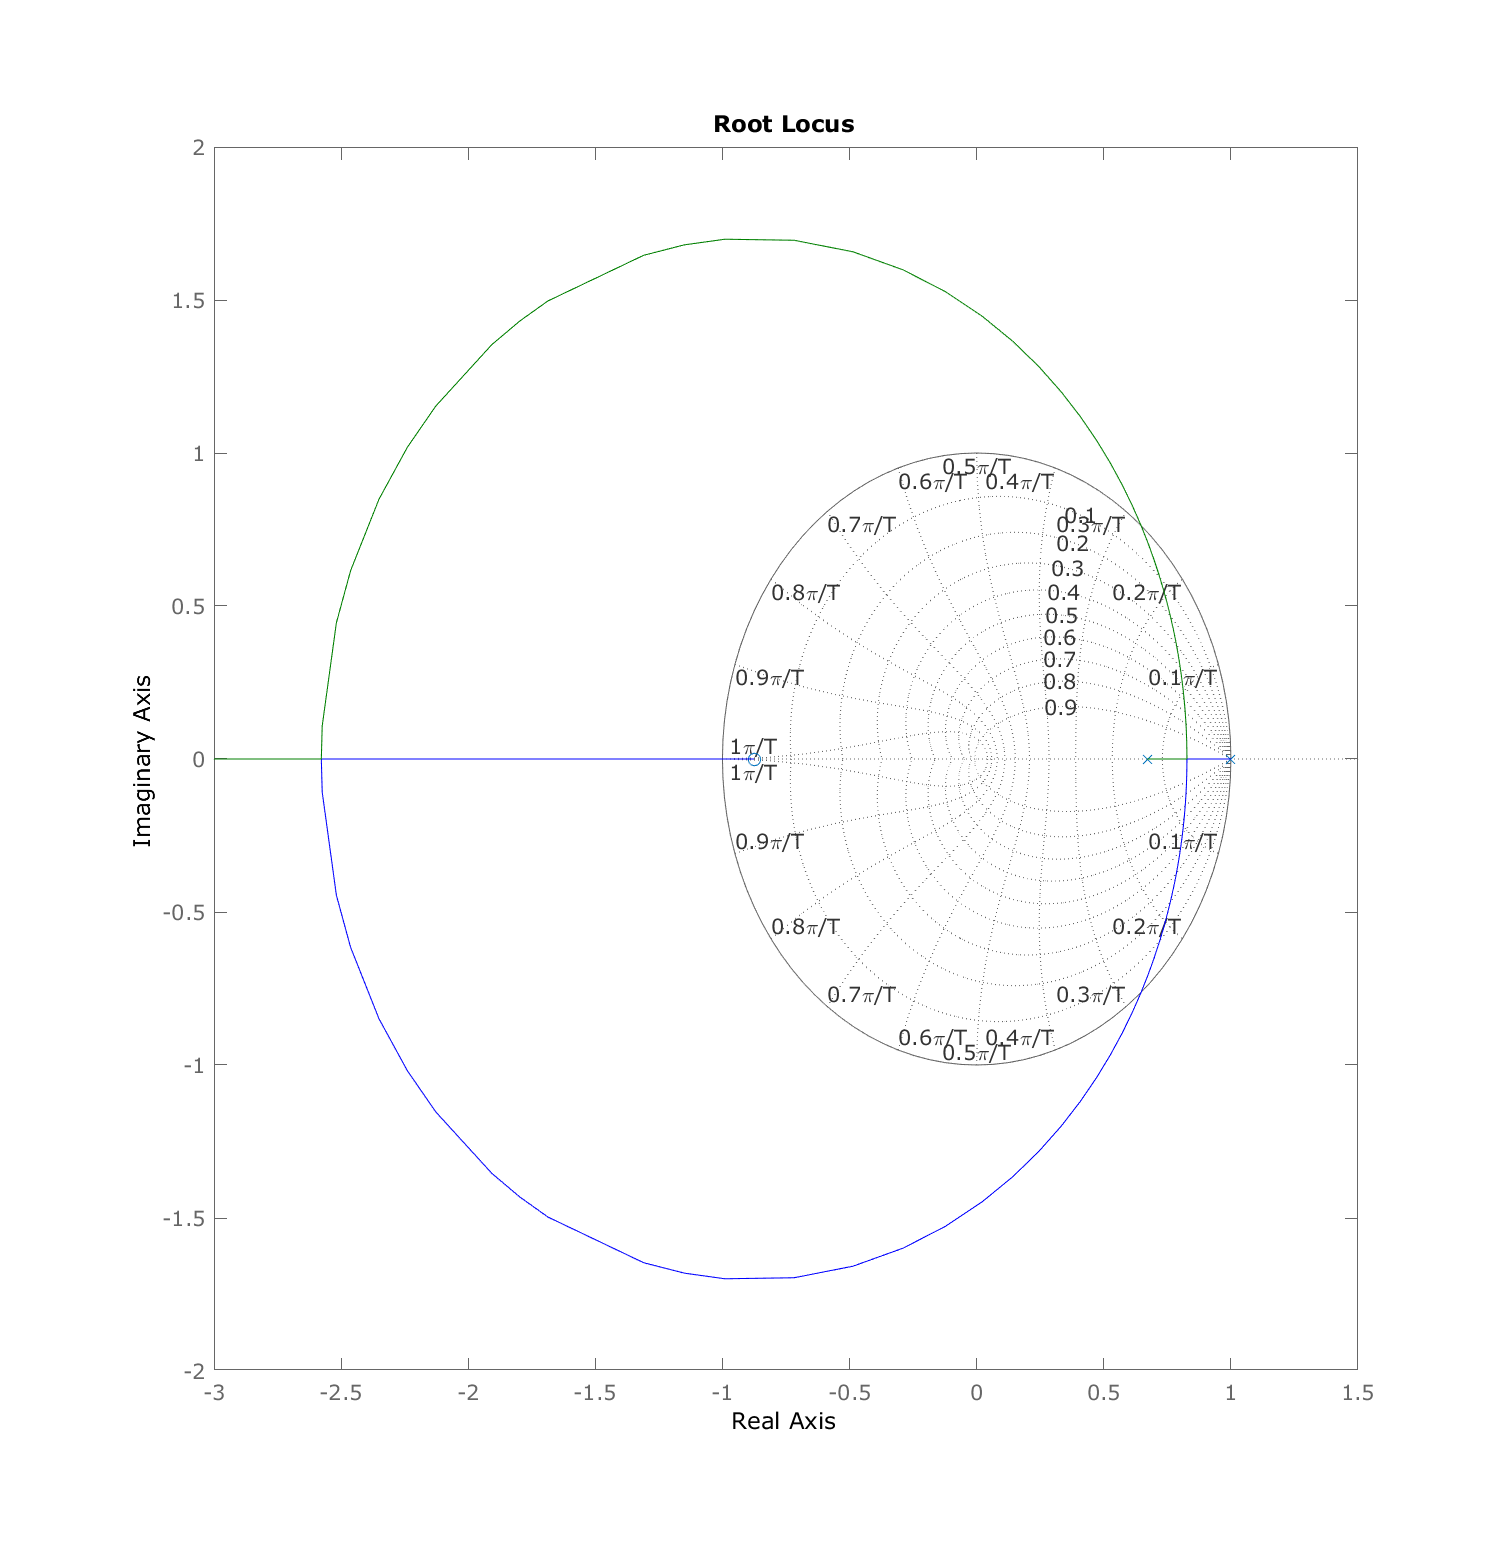
\includegraphics[width=0.9\linewidth]{img/exsim3-rlocus-g2.png}
    \caption{LGR sem o controlador}
    \label{fig:ex3-rlocus-g2}
\end{figure}

A partir do gráfico \ref{fig:ex3-rlocus-g2} temos que o LGR da planta sem o controlador já intercepta a curva dada por $\zeta = 0.5$, no entanto é necessário verificar se o tempo de acomodação já cumpre os requisitos.

%%\section{Conclusão}

% ------------------------------------------------------------------------------

% Referências
\addcontentsline{toc}{section}{Referências} % Adiciona linha no indice
\bibliographystyle{abbrv} % Define Estilo e gera bibliografia
\bibliography{references} % Adiciona Arquivo com Referências

% Acrescentadas no arquivo references.bib
% para usa-las no texto basta usar \citep{}
% para citar sem usar no texto basta usar \nocite{}
\nocite{sympy}
\nocite{pythontex}
\nocite{matlabcontrol}
\nocite{matlabsymbolic}

% ------------------------------------------------------------------------------
\newpage
\section*{Anexos}
\addcontentsline{toc}{section}{Anexos} % Adiciona linha no indice
\subsection*{Python}

Para os cálculos e demonstrações foi utilizado o pacote \textit{Python}\TeX\ \cite{pythontex} para o \LaTeX\ em conjunto da bibliteca \textit{sympy}\cite{sympy}. Segue o script completo em python:

\inputminted[xleftmargin=15pt,linenos,frame=single,framesep=5pt,breaklines=true]{python}{../python/exsim3.py}

\newpage
\subsection*{Matlab}

%\subsubsection*{Parte 1}
Para o desenho dos gráficos e simulações foi utilizado o \textit{Matlab} em conjunto das toolbox \textit{Control System}\cite{matlabcontrol} e \textit{Symbolic Math}\cite{matlabsymbolic}. Segue o código referente usado

\inputminted[xleftmargin=15pt,linenos,frame=single,framesep=5pt,breaklines=true]{matlab}{../matlab/exsim3.m}

%\subsubsection*{Parte 2}
%Na segunda parte foi utilizado uma versão modificada do script em \textit{Matlab} fornecido pelo professor:
%\inputminted[xleftmargin=15pt,linenos,frame=single,framesep=5pt]{matlab}{../matlab/exsim2/exsim2script.m}



% ------------------------------------------------------------------------------
\end{document}
